\textbf{See the instruction for questions \inteval{\value{question}+1} to \inteval{\value{question}+2}.}

General instruction (if any) goes here.

\begin{figure}[H]
\centering
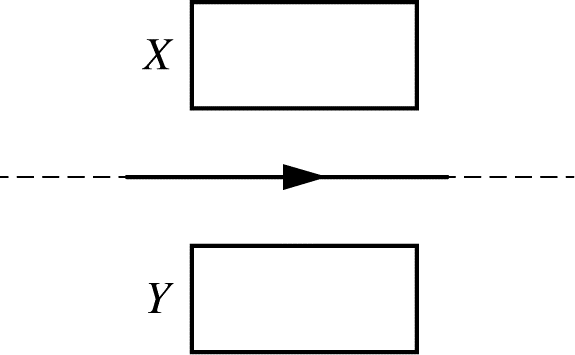
\includegraphics[scale=0.25]{images/img-015-041.png}
\end{figure}
Two identical rectangular conducting loops and a very long, straight wire lie in the plane of the page, as shown above. The loops are equal distances from the wire, and there is a current to the right in the wire.

% Multiple Choice Question 34
\begin{questions}\setcounter{question}{33}\question
If the current in the wire is decreasing, what is the direction of the induced current, if any, in each of the loops?

\tabto{0.75cm}\underline{Loop $X$}
\tabto{5.00cm}\underline{Loop $Y$}

\begin{choices}
\choice Counterclockwise \tabto{4.25cm} Clockwise
\choice Counterclockwise \tabto{4.25cm} Counterclockwise
\choice Clockwise        \tabto{4.25cm} Counterclockwise
\choice Clockwise        \tabto{4.25cm} Clockwise
\choice None             \tabto{4.25cm}  None
\end{choices}\end{questions}

% Multiple Choice Question 35
\begin{questions}\setcounter{question}{34}\question
If the current in the wire is constant and the wire is moved toward loop $X$, what is the direction of the induced current, if any, in each of the loops?

\tabto{0.75cm}\underline{Loop $X$}
\tabto{5.00cm}\underline{Loop $Y$}

\begin{choices}
\choice Counterclockwise \tabto{4.25cm} Clockwise
\choice Counterclockwise \tabto{4.25cm} Counterclockwise
\choice Clockwise        \tabto{4.25cm} Counterclockwise
\choice Clockwise        \tabto{4.25cm} Clockwise
\choice None             \tabto{4.25cm}  None
\end{choices}\end{questions}

